\scanpage{74}
The system of inequalities \textcircled{17} (for variable $m,n$) and \uline{the consequence (15)}, seem to be the inequalities, the strongest possible bounding the \inserted{system of} $\rho_i(u+v)$ from above in terms of the $\rho_i(u)$, $\rho_i(v)$. Let us note that one could deduce \deleted{\unsure{in the same way}} \inserted{directly} inequality \uline{(15)} from inequality \uline{(12)} which it \uline{generalizes}, \uline{for this let us point out} the \deleted{\unsure{proposition}}

\uline{Proposition 4} If $u\in L_0(E,F)$, \deleted{\unsure{and}} $n$ is an integer $>0$, we have

\[
\begin{array}{@{}l@{\qquad}l@{}}
(18) & \displaystyle \deleted{d}\prod_1^n(1+\rho_i(u))=\operatorname*{Sup}_{\substack{v_n\in L(F,E)\\\lVert v_n\rVert\leq1\\\operatorname{rang}v_n\leq n}}\det(1+v_nu)
\end{array}
\]

This \deleted{proof} \inserted{formula} is proved as (17), \deleted{\unsure{one can even}} \inserted{\deleted{\unsure{by}} the} reasoning is \deleted{\unsure{=|m} \unsure{slight\textsuperscript{ly}|slightly} more \unsure{simple}} \inserted{left to the reader}

\figure{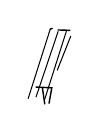
\begin{tikzpicture}[x=1mm,y=1mm,line cap=round]
\draw[line width=.13mm] (0,0)--(2.8,8.8) (1.0,.2)--(3.8,8.5) (2.1,-.1)--(4.9,8.7) (3.7,3.6)--(5.4,7.9);
\draw[line width=.18mm] (2.8,8.8)--(3.05,8.9) (3.8,8.7)--(5.3,8.65) (1.0,1.45)--(3.0,1.35)--(2.65,-.6) (1.8,1.4)--(2.1,-.7);
\end{tikzpicture}}

\margin{75}
